\chapter{Comparison of Methods}
\section{Introduction}
This chapter takes a comparative look at the six metaheuristics, Random Search (RS), Hill Climbing (HC), Simulated Annealing (SA), Genetic Algorithms (GA), Evolutionary Strategies (ES) and Evolutionary Programming (EP).
We first present a summary of the results, showing success rates for each of the Symbolic Integration, Santa Fe, Blocks and  Symbolic Regression problems.

We also attempt to profile aspects of the search space presented to the metaheuristics and summarise some of the characteristics of the problems and their solutions.

The most successful of the metaheuristics, the three population based search strategies, GA, EP and ES  are analysed and compared, first comparing GA and ES before turning our attention to EP and GA.

Finally, we look at wrapping and search for characteristics of the problems or aspects of the grammars that might influence it.

\section{Comparing the results}
Table~\ref{all_results_analysis_table} provides a summary of success rates for all problems and metaheuristics. GA and ES emerge as the strongest of the search strategies, with the population based methods in general showing a clear advantage over the local search based approaches of HC and SA.

 The results indicate that Symbolic Regression has a high degree of difficulty, remaining unsolved by RS, HC and SA. 
HC would appear to be the least successful of all of the search strategies evaluated, with RS emerging as the most successful of the non-population based search methods.



\begin{table}[h]
\begin{center}
\begin{tabular}{|l|l|l|l|l|}
\hline
Metaheuristic & Sym Int & Santa Fe & Blocks & Sym Reg  \\
\hline

Random Search &              40\%    &  30\%    &  24\%    & 0\%   \\
Hill Climbing &               8\%    &  15\%    &  17\%    & 0\%    \\
Simulated Annealing &        11\%    &  21\%    &  13\%    & 0\%    \\
Genetic Algorithms &        100\%    &  81\%    &  99.5\%  & 36\%   \\
Evolutionary Strategies &    95\%    &  63\%    &  96\%    & 25\%   \\
Evolutionary Programming  &  94\%    &  73\%    &  95\%    & 25\%   \\

\hline
\end{tabular}
\caption{\label{all_results_analysis_table} A Summary of Success Rates for all Metaheuristics.}
\end{center}
\end{table}



\section{Characteristics of the Search Space}
The results in the previous section show a performance benefit in using population based methods (GA,EP and ES). In order to understand the aspects of the search space that might explain the limitations of the local search methods we profiled the search space for each of the problems.

The profiles for each of the problems consist of all of a successful solution's immediate neighbours within a hamming distance (i.e. a single codon difference in the genome) of one.  The hamming distance of one was chosen as the basis for this profile because it represents the smallest possible unit of change  between one solution and another. Only expressed codons are changed, the unexpressed tail is removed from the genome before the neighbourhood is generated. Once all neighbours have been generated the unexpressed tail is re-attached to each of the individuals in the neighbourhood. This re-attached tail allows them utilise the ripple effect to form new solutions. It should be noted that neighbours in this context are not ancestors of successful solutions, rather they are generated from successful solutions using the method outlined above. The objective here is to provide some insight into the sensitivity of successful genomes to change.

The plots shown are a composite of all solutions from all of the trials. This data is also presented in summary form in Table~\ref{neighbours_table} where we show the percentage fall off in fitness of the immediate neighbourhood. So, for example, in the case of Santa Fe, 22.30\% of the neighbours also  achieve maximum fitness, while 0.49\% have a score that is within 20\% of maximum fitness. 



\begin{table}[h]
\begin{center}
\begin{tabular}{|l|l|l|l|l|l|l|}
\hline
&\multicolumn{6}{|l|}{Percentage Drop in Fitness (0 - 50\%)}\\
\hline
Problem & 0\%  & 10\% & 20\% & 30\% & 40\% & 50\% \\
\hline
\hline
Santa Fe & 22.3\%  & 0.11\% & 0.49\% & 0.15\% & 0.36\% & 2.08\% \\
Sym Integration & 7.09\% & 0.02\% & 0.0\% & 0.0\% & 0.0\% & 0.0\%  \\
Sym Regression & 4.39\% & 1.38\% & 2.09\% & 1.17\% & 2.16\% & 1.91\% \\
Blocks Stacking & 33.0\% & 0.55\% & 0.96\% & 12.64\% & 2.61\% & 6.55\% \\
\hline
&\multicolumn{6}{|l|}{Percentage Drop in Fitness (50 - 100\%) }\\
\hline
Problem & 50\% & 60\% & 70\% & 80\% & 90\% & 100\% \\
\hline
\hline
Santa Fe & 2.08\% & 0.72\%  & 4.21\% & 8.82\% & 35.62\% & 25.15\%  \\
Sym Integration & 0.0\% & 0.02\% & 0.04\% & 2.36\% & 83.38\% & 7.04\% \\
Sym Regression & 1.91\% & 3.43\% & 5.56\% & 7.75\% & 56.48\% & 13.69\% \\
Blocks Stacking & 6.55\% & 11.58\% & 5.82\% & 0.23\% & 0.0\% & 25.50\% \\
\hline
\end{tabular}
\caption{\label{neighbours_table} Percentage fall off in Fitness of Immediate Neighbours for all Problems.}
\end{center}
\end{table}





\begin{figure}[]
\centerline{\hbox{
\psfig{file=Chapter11/graphs/santafe_neighbourhood.ps,width=4in}}}
\caption[Neighbourhood of a Solution for The Santa Fe Trail Problem.]{ Neighbourhood of a Solution for The Santa Fe Trail Problem. The graph shows the immediate neighbourhood of solutions. The Y-axis shows the fitness while the X axis displays the neighbours sorted in descending order.}
\label{santafe_neighbourhood}
\end{figure}


\subsection{Santa Fe Trail}
The plot for Santa Fe shown in Figure~\ref{santafe_neighbourhood}  shows a sharp fall of in fitness from a plateau of maximum fitness. An examination of all of the Santa Fe solutions found during the trials shows that, on average, 22.3\% of neighbours (see Table~\ref{neighbours_table}) of a Santa Fe solution will also have perfect fitness. Of these 22.3\% perfectly fit neighbours, 20\% are identical mapping to the same solution and following the same sequence in selecting productions. 

The average number of expressed codons in a solution for Santa Fe is 51, which is much longer than the nine required for the minimal successful solution. One of the structures that tends to create some of the longer solutions is the multiple nesting of the \emph{$if(trail.food\_ahead())$} conditional.  

The profile of the Santa Fe neighbourhood might help explain why the local search approaches experiences difficulty, within the neighbourhood of a solution there are points of very low fitness, with no progressive slope for the algorithms to climb. An approach that attempts to fine tune a solution through gradual exploration of the immediate neighbourhood is always likely to perform poorly.

Santa Fe shows a reduction in performance when \emph{Genetic Code Degeneracy} is reduced by restricting  the range of codon values used to the maximum number of production rules in the grammar (i.e from 256 to 3). A trial of 1000 runs using Random Search with a maximum codon value of two saw the performance drop to 4\% from the original success rate of 30\%. Increasing the maximum codon value by one to three causes the performance recover to the original 30\%.

This sensitivity is possibly a consequence of the simple modulo function (see Section~\ref{modulo}) used by GE. This rule selection function is degenerate allowing many codon values to map to the same choice of rules. One of the consequences of this is a linkage between production rules belonging to different non-terminal symbols. This linkage, which is strongly influenced by layout and sequencing of the rules introduces a bias into the search process~\cite{keijzer}.   

Degeneracy also acts toward the preservation of the functionality of the phenotype while allowing unrestricted exploration of the genotypic search space as evidenced by increases in the number of invalid individuals when it is removed~\cite{ge_book}~\cite{mike_thesis}. 

\subsection{Symbolic Integration}
An analysis of the immediate neighbourhood of solutions for Symbolic Integration (see Figure~\ref{symint_neighbourhood}) shows a different profile to that of Santa Fe, we again see fitness fall off sharply from a peak of maximum fitness, however the plateau of maximum fitness is greatly reduced. Just over 7\% of the immediate neighbours of solutions retain maximum fitness, indeed Table~\ref{neighbours_table} shows that over 83\% of all neighbours have values that have fallen by 90\%.
The implications of this is that area of the global maxima (that is, the correct answer) is significantly smaller than in the Santa Fe problem, so relatively small changes in individuals in this neighbourhood are considerably less likely to result in a global maxima. The effects of this can be seen in table~\ref{all_results_analysis_table} where the performance of HC and SA have both dropped. 

Symbolic Integration shows a less pronounced effect when the range of the codon value is restricted to reduce the impact of \emph{Genetic Code Degeneracy} . We see the success rate for Random Search fall from 40\% to 27\% when the maximum value of the codon is reduced from 255 to two. 
 
\begin{figure}[]
\centerline{\hbox{
\psfig{file=Chapter11/graphs/symint_neighbourhood.ps,width=4in}}}
\caption[Neighbourhood of the Solution for The Symbolic Integration Problem.]{ Neighbourhood of the Solution for The Symbolic Integration Problem. The graph shows the  immediate neighbourhood of solutions. The Y-axis shows the fitness while the X axis displays the neighbours sorted in descending order.}
\label{symint_neighbourhood}
\end{figure}


\subsection{Blocks}
Figure~\ref{blocks_neighbourhood}  shows a rather different profile to that of the other problems, we see a more gradual slope to maximum fitness. This profile would tend to suggest that approaches like HC and SA should perform strongly relative to RS, and while we do see less of a performance gap between RS and HC/SA, RS still scores better. This may partly be explained by the scoring scheme used in the Blocks problem (see Section~\ref{blocks_scores}), which makes it quite easy to score a relatively high fitness level for solutions that fall short of correctly stacking the blocks. 

When the range of codon values is reduced in the Blocks problem we see similar results to that of Santa Fe with the success rate for Random Search based trials fall from 24\% to 10\%.

Solutions for the Blocks problems tend to be quite long requiring 57 codons on average, which is longer than the number of codons required for any of the other problems and also longer than the shortest found for this problem which required 20 codons. The aspects of the grammar that contribute to this long length are redundant sequences of the negation operator (!) and some nesting of the \emph{Do Until} construct. 


\begin{figure}[]
\centerline{\hbox{
\psfig{file=Chapter11/graphs/blocks_neighbourhood.ps,width=4in}}}
\caption[Neighbourhood of a Solution for The Blocks Stacking Problem.]{ Neighbourhood of a Solution for The Blocks Stacking Problem. The graph shows the immediate neighbourhood of solutions. The Y-axis shows the fitness while the X axis displays the neighbours sorted in descending order.}
\label{blocks_neighbourhood}
\end{figure}


\begin{figure}[!hbp]
\centerline{\hbox{
\psfig{file=Chapter11/graphs/symreg_neighbourhood.ps,width=4in}}}
\caption[Neighbourhood of a solution for The Symbolic Regression Problem.]{ Neighbourhood of a solution for The Symbolic Regression Problem. The graph shows the immediate neighbourhood of solutions. The Y-axis shows the fitness while the X axis displays the neighbours sorted in descending order.}
\label{symreg_neighbourhood}
\end{figure}

\subsection{Symbolic Regression}
The neighbourhood of a Symbolic Regression problem is similar to that of Symbolic Integration, showing a sharp isolated peak with a more gradual yet pronounced fall off in fitness as shown in Figure~\ref{symreg_neighbourhood}. Solutions for Symbolic Regression require 49 codons on average, which is less than the number required for Blocks or Santa fe. 

ES was used to evaluate Symbolic Regression's sensitivity to changes in the range of codon values. We see evidence of a strong dependency to the original range of values as suggested by the drop in success rates falling from 25\% to 1\% when the maximum genome value is set to two. This contrasts with the results from the Symbolic Integration which shares the same grammar. 
 



\section{Analysis of Solution Lengths}
The average numbers of expressed codons in a solution are presented in Table~\ref{all_characteristic_analysis_table} showing Blocks as the problem requiring the largest number at 57, Symbolic Integration requires fewest at 16 while Santafe and Symbolic Regression require 51 and 49 respectively. The solution lengths for Blocks and Santa Fe are quite long when one considers the shortest solutions found for these problems, for example Blocks can be solved with a genome length of 20 and Santa Fe only requires 9 codons for success. The factors contributing to this tendency toward longer genome lengths will be explored further in Section~\ref{grammar_wrap}. 



\begin{table}[h]
\begin{center}
\begin{tabular}{|l|l|l|l|l|}
\hline
Metaheuristic             & Sym Int & Santa Fe & Blocks & Sym Reg  \\
\hline
Random Search             & 14      & 46       & 69     & n/a   \\
Hill Climbing             & 15      & 47       & 77     & n/a  \\
Simulated Annealing       & 19      & 48       & 91     & n/a \\
Genetic Algorithms        & 13      & 43       & 49     & 42  \\
Evolutionary Strategies   & 18      & 53       & 39     & 49  \\
Evolutionary Programming  & 19      & 74       & 71     & 57 \\
\hline
Average                   & 16      & 51       & 66     & 49 \\
\hline
\end{tabular}
\caption{\label{all_characteristic_analysis_table} A Summary of Successful Solution sizes for all Metaheuristics.}
\end{center}
\end{table}

\section{Comparing ES, EP and GA}

While ES and GA share many similarities, with both approaches employing both mutation and recombination operators there are a number of significant differences in their approach. The selection strategy used by ES in these trials was the plus strategy (see Section~\ref{es_selection_strategies}), which selects  the best individuals from the union of parents and offspring  to survive. Selection in this GA consists of \emph{remainder stochastic sampling without replacement} with steady state populations. The mutation operator in GA is based on the probability of mutating an individual bit in a codon whereas ES uses mutation at the codon level using a mutation rate that evolves as a strategy variable from generation to generation. 

ES uses fixed length genomes while GA uses variable length genomes that can grow in length under the influence of the crossover and duplication operators. Finally, the population sizes differs with GA using a larger population size of 500 against a typical ES population size of 50.

EP and GA also have a number of significant differences, with EP using  a population size of 50 against 500 for GA. EP also uses a fixed length genome, while GA uses variable length genomes. The selection methods differ in that GA uses \emph{remainder stochastic Sampling without replacement} with steady state populations while EP uses a \emph{tournament based} selection strategy to select individuals from a combined population of parents and offspring.

The mutation operator in GA is based on the probability of mutating an individual bit in a codon whereas EP uses mutation at the codon level using a mutation rate that evolves as a strategy variable from generation to generation. 

Rows three to six of Table~\ref{all_results_analysis_table} show the results from the original ES, EP and GA trials, while the results from these methods are reasonably close, overall, GA shows a statistically significant advantage over ES and EP. This is most apparent on the Santa Fe and Symbolic Regression problems.




\section{Fixed and Variable length Gemones on EP and GA}

\begin{table}[h]
\begin{center}
\begin{tabular}{|l|l|l|l|l|}
\hline
Metaheuristic          & Sym Int      & Santa Fe       & Blocks         & Sym Reg \\
\hline
GA (pop 500)           &              &                &                &                \\
no crossover           & 11\%         & 18.9\%         & 4.7\%          & 0.59\%         \\
EP (pop 50)            & 94\%         & 73\%           & 95\%           & 11\%           \\
\hline
\end{tabular}
\caption{\label{ep_ga} Results from a Comparative Analysis of GA with no crossover and EP.}
\end{center}
\end{table} 

In Section~\ref{operator_removal} we looked at the performance of GA with the crossover operator removed. Table~\ref{ep_ga} shows the results of EP alongside those of GA with crossover removed, revealing a significant difference in the performance of EP over GA.

While GA and EP have many differences in their structure, in this scenario they both operate without the benefit of crossover, relying on mutation to create new individuals. One of the characteristics that distinguishes them is the use of fixed length genomes by EP and variable length genomes by GA. 

The normal operation of the GA algorithm uses randomly generated lengths of genomes to create the initial population. EP differs in this respect by using fixed length genomes of a specific pre-determined size. Introducing fixed length genomes into GA sees a significant improvement in its performance when the crossover operator is omitted. Conversely, the introduction of variable length genomes to EP does not adversely influence its success rate, indeed Symbolic Regression shows a significant increase in performance from 11\% to 20\%. These results are shown in Table~\ref{ep_ga_genome}, with rows one and two showing the original success rates and three and four showing the changes when fixed length genomes are introduced to GA and variable length genomes are used in EP. 

\section{Experimental Conditions}
The parameters used to configure fixed length GA for these trials are presented in Table~\ref{ga_fixed_param_table}. Variable length EP used the parameters presented in Table~\ref{ep_variable_param_table}. The variation in EP individuals is established at the initial creation of the population. Because EP uses only mutation the length of the individuals does not change beyond the initial generation. 



\begin{table}[h]
\begin{center}
\begin{tabular}{|l|l|l|l|l|}
\hline
Parameter &\multicolumn{4}{l|}{Problems}\\
\cline{2-1} \cline{3-1} \cline{4-1} \cline{5-1} 
 & Sym Int & Santa Fe & Blocks & Sym Reg  \\
\hline
Number of Trials & 1000 & 1000 & 1000 & 1000 \\
Number of Objective & & & & \\ 
Function Evaluations  & 25000 & 25000 & 25000 & 25000  \\
Initial Genome Length  & 100 & 100 & 100 & 200  \\
Population Size  & 500 & 500 & 500 & 500  \\
Number of Generations  & 50 & 50 & 50 & 50  \\
Probability of Swap  & .01  & .01  & .01 & .01   \\
Probability of Duplication   & .01  & .01  & .01 & .01  \\
Probability of Crossover & 0  & 0  & 0 & 0  \\
Probability of Mutation & .01  & .01  & .01 & .01  \\
\hline
\end{tabular}
\caption{\label{ga_fixed_param_table} Parameters used to configure the Fixed Length Genetic Algorithm.}
\end{center}
\end{table}



\begin{table}[h]
\begin{center}
\begin{tabular}{|l|l|l|l|l|}
\hline
Parameter &\multicolumn{4}{l|}{Problems}\\
\cline{2-1} \cline{3-1} \cline{4-1} \cline{5-1} 
 & Sym Int & Santa Fe & Blocks & Sym Reg \\
\hline
Number of Trials & 1000 & 1000 & 1000 & 1000  \\
Number of Objective & & & & \\ 
Function Evaluations  & 25000 & 25000 & 25000 & 25000  \\
Initial Genome Length Range & 10-100 & 10-100 & 10-100 & 10-100  \\
Population Size  & 50 & 50 & 50 & 50  \\
Number of Generations  & 500 & 500 & 500 & 500  \\
\hline
\end{tabular}
\caption{\label{ep_variable_param_table} Parameters used to Configure Evolutionary Programming.}
\end{center}
\end{table}

\begin{table}[h]
\begin{center}
\begin{tabular}{|l|l|l|l|l|}
\hline
Metaheuristic          & Sym Int      & Santa Fe       & Blocks         & Sym Reg \\
\hline

GA                     &              &                &                &                \\
no crossover           & 11\%         & 18.9\%         & 4.7\%          & 0.59\%         \\
\hline
EP                     & 94\%         & 73\%           & 95\%           & 11\%           \\
\hline
\hliness
GA                     &              &                &                &        \\
no crossover           & 74\%         & 54\%           & 46\%           & 33\%    \\
Fixed Length           & (+63\%)      & (+35.1\%)      & (+41.3\%)      & (+32.4\%)    \\
\hline
EP                     & 94\%         & 62\%           & 91\%           & 20\%        \\
Variable Length        & (0\%)        & (-11\%)        & (-4\%)         & (+9\%)   \\
\hline
\end{tabular}
\caption{\label{ep_ga_genome} Analysis of the Impact of Fixed and Variable Length Genomes on GA without crossover and EP.}
\end{center}
\end{table} 


\section{Wrapping}
One curious aspect of these results in the prominence of wrapping in solving some problems and the degree to which the proportion of solutions using wrapping varies between metaheuristics. Symbolic Regression has little dependence on wrapping, appearing only when GA is used,  while Santa Fe and Blocks show high proportions of wrapping in solutions with Santa Fe using wrapping on average in 46\% of all solutions while Blocks has an even higher proportion at 52\%. On average Symbolic Integration uses wrapping in only 0.16\% of solutions, indeed wrapping does not appear in any Symbolic Integration solutions found by RS, ES or EP.


We created a set of trials for the Symbolic Integration in order to determine if the absence of wrapping in Symbolic Integration is due to the fact that the required number of expressed genomes is low (16) relative to the length of solutions typically generated by the various search strategies.  The initial genome length was set to 10, which is six codons shorter than the 15 codons required on average for a successful Symbolic Integration solution. As a control we ran a similar trial for Santa Fe with the genome length set at 38, also six shorter than the average number required for a solution. The selection of these particular lengths was arbitrary, the only criteria being that GE would be forced to wrap in the majority of cases.

Random Search was used as the search mechanism for these trials in which Santa Fe scored a 29\% success rate, not significantly different than the score achieved in the original Random Search trials (30\%). Symbolic Integration, however, was successful in none of the 500 runs.

The results of these trials indicate that the absence of wrapping in the case of Symbolic Integration is not due to the short length of genome required to solve this particular problem, when the problem is forced to use wrapping it fails, which is contrasted with Santa Fe which readily copes with the short Genome lengths by employing wrapping to create solutions. These results would seem to suggest that the tendency to use wrapping is linked to the nature of the problem and/or its associated grammar.

\subsection{Grammars and Wrapping}
\label{grammar_wrap}Table~\ref{all_wrapping_analysis_table} provides a summary of the proportion of wrapping associated with each of the problems. Symbolic Integration and Symbolic Regression show little, if any, dependency on wrapping, while Blocks and Santa Fe have a significant amount of solutions that use wrapping. Symbolic Integrations and Symbolic Regression both use the same grammar, which provides some fundamental building blocks ($x,+,-,*,sin$) to build the target expressions $f(x) = Sin(x) + x^2 + x$ and $x^4 + x^3 + x^2 + x$. The solutions for these expressions show a high degree of repetition, often combining long sequences of the combination $x * x$, the repetitive nature of this could be one of the factors that contributes against wrapping appearing in solutions.



\begin{table}[h]
\begin{center}
\begin{tabular}{|l|l|l|l|l|}
\hline
Metaheuristic            & Sym Int & Santa Fe & Blocks & Sym Reg  \\
\hline
Random Search            &  0\%    & 43\%    & 41\%   & n/a   \\
Hill Climbing            &  0\%    & 80\%    & 70\%   & n/a  \\
Simulated Annealing      &  0\%    & 50\%    & 66\%   & n/a \\
Genetic Algorithms       &  1\%    & 91\%    & 85\%   & 1\%  \\
Evolutionary Strategies  &  0\%    & 0\%     & 0\%    & 0\%  \\
Evolutionary Programming &  0\%    & 25\%    & 46\%   & 1\% \\
\hline
Average                   & 0.16\%    & 48\%    & 51\%   & 1\% \\ 
\hline
\end{tabular}
\caption{\label{all_wrapping_analysis_table} Proportion of Wrapping appearing in Successful Solutions for all Metaheuristics.}
\end{center}
\end{table}


\subsection{Impact of Conditionals on Wrapping}
Another distinction between the grammars is the presence of conditionals,  \emp{\begin{verbatim} DO  <code> UNTIL <code> ODU \end{verbatim}} \noindent in the case of Blocks and \emp{\begin{verbatim} if(food_ahead()){ <line> else <line>}\end{verbatim}} \noindent for the Santa Fe problem. The solutions that use wrapping typically have multiple nested loops using these constructs. These multiply nested loops are often redundant in that they add nothing to the actual logical flow of the program but they may provide a means of consuming codons in a way that allows wrapping provide solutions. A example of this nesting from a Santa Fe solution is shown below.


\begin{verbatim}
if(trail.food_ahead())
   {
   if(trail.food_ahead())
      {
      if(trail.food_ahead())
         {
         if(trail.food_ahead())
            {
            if(trail.food_ahead())
               {
               trail.move()
               }
            else
               {
               trail.move()
               }
            }
         else
         .................
\end{verbatim}

In order to determine if the presence of conditionals in a grammar increases the probability of wrapping we introduced a conditional into a grammar used for solving the Symbolic Integration problem. This grammar was a simplified version of the grammar presented in Section~\ref{sym_int_grammar}. 

\small
\begin{verbatim}
<expr>         :: ==  <expr><op><expr> | <pre-op>(<expr>) | <var> 
<var>          :: == X  	                                           
<op>           :: == + | - | / | *                            
<pre-op>       :: == sin | cos         

\end{verbatim}
\normalsize  

In this simplified form the order of some of the production rules were deliberately changed to first determine if this in itself had an impact. We first performed a 1000 runs with the new grammar without any conditionals present. We used RS as the search mechanism and found that wrapping did not appear in any of the solutions found. When the problem was forced to use wrapping by using short genome lengths it failed on every occasion to find a solution.

We then introduced a simple conditional into the grammar. The conditional took the form of \begin{verbatim} IF (1) THEN <expr> ELSE <expr> ENDIF \end{verbatim}\noindent This had the effect of allowing solutions to be enclosed in a conditional construct that always defaulted to the first expression by virtue of the fact that the \emph{IF} statement was always true. The complete grammar took the following form:

\small
\begin{verbatim}
<expr>         :: ==  <expr><op><expr> 
                    | <pre-op>(<expr>)
                    | <var>
                    | <control>
<control>      :: IF ( 1 ) THEN  <expr>  ELSE  <expr>  ENDIF   
<var>          :: == X  	                                           
<op>           :: == + | - | / | *                            
<pre-op>       :: == sin | cos         

\end{verbatim}
\normalsize  
 
When we again conducted a 1000 runs with RS using this new grammar we found that wrapping appeared in 5\% of the solutions found. When wrapping was forced on the method by using short genome lengths it managed a success rate of 14\%. While these results would suggest a possible relationship between wrapping and the presence of conditionals in a grammar much more research is required to fully understand the nature of the relationship. 

It is also important to remember that the operators also influence the probability of wrapping appearing in solutions. This is most evident in the contrasting results of EP and ES, where we saw wrapping appear in EP  but not in ES. Significantly, both methods used fixed length genome that were sufficiently longer than the required number of codons for a successful solution. These results would suggest that something in the EP approach, perhaps the absence of recombination (which is present in ES) forced the method toward longer genome lengths utilising wrapping to solve the problem. 

There is probably no simple single explanation for the emergence  of wrapping in some problems.  A detailed cross comparison of the codons of successful solutions shows no obvious patterns in either those that use wrapping and those that do not. The results of the research on the Symbolic Integration grammar, which saw wrapping emerge when we included a simple conditional in the grammar, suggests that an area for future research would be an analysis of the correlation between the presence of these type of constructs and the probability of wrapping. This could be supported by the selection of problems and the construction of grammars that are likely to have both condition constructs and high levels of repetition. 



\section{Summary}
In this chapter we have taken a comparative look at the results featured in the previous chapters. These results show a strong performance by the population based search strategies like GA, EP and ES, while the local search approach of HC and SA have limited success. Curiously, RS performs strongly on three of the problems, out-scoring HC and SA.

We looked also at the problems Symbolic Integration, Santa Fe, Symbolic Regression and Blocks, attempting to offer some insight into the search space in the immediate neighbourhood of solutions. The profiles of three of the problems suggested a terrain that would be difficult for local search metaheuristics like HC and SA.

GA, ES and EP were contrasted and compared, looking in particular at the impact of fixed and variable length genomes on GA and EP.

Finally, we looked at wrapping and attempted to understand why it appeared so prominently in two of the problems. We found that the presence of wrapping is not due solely to the length of genome solutions as demonstrated by Symbolic Integration which failed to find any solutions when forced to use wrapping. As a basis for some future work we suggested research that looked at particular constructs in the grammars in particular, loops based on conditionals and large amounts of repetition in solutions.























